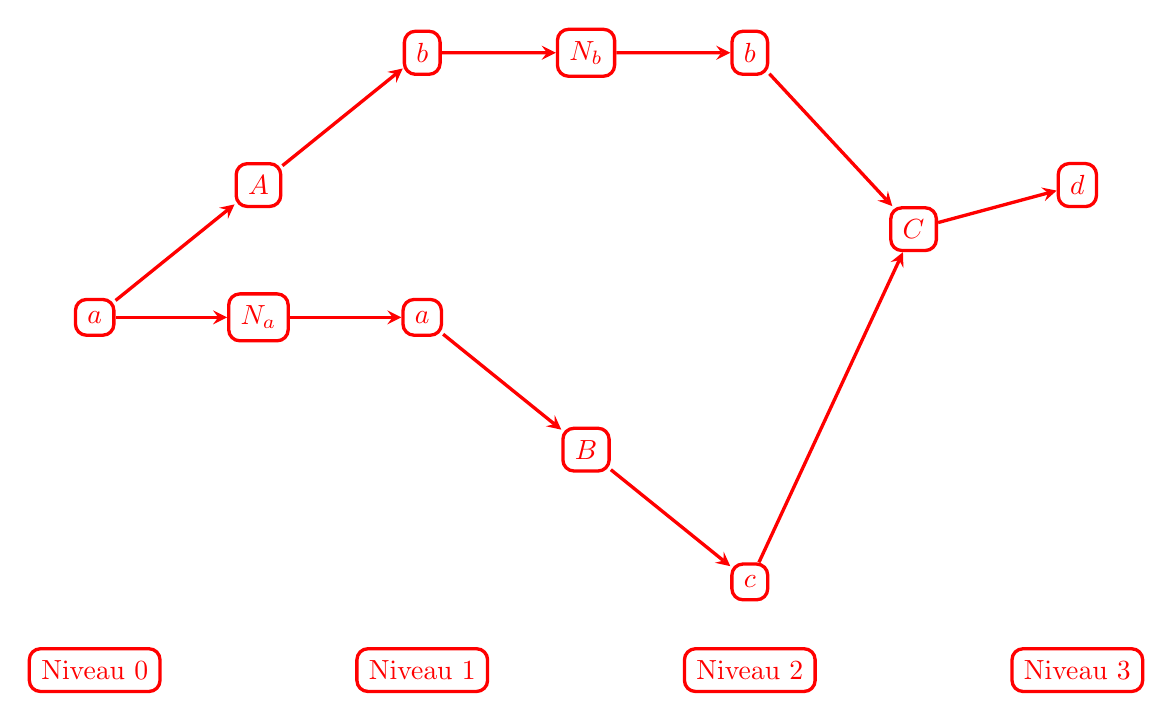
\begin{tikzpicture}
   [  yscale=0.7, xscale=1.3, scale=1.6,
      pre/.style={<-,shorten <=0pt,>=stealth},
      post/.style={->,shorten >=0pt,>=stealth},
      base/.style={draw, very thick,color=red},
      maintienFluent/.style={base},
      ajoutFluent/.style={base},
      texty/.style={base, rounded corners,inner sep=1ex}]
% =========================================================================
% =============================== LE SCHEMA ===============================
% =========================================================================

\begin{scope}
    \tikzstyle{every node}=[texty] %%
     \node (n0)      at (0,0)            {$a$};

      \node (n11)     at (1,1.5)          {$A$}
         edge [pre,ajoutFluent]        (n0);
      \node (n10)     at (1,0)            {$N_a$}
         edge [pre,maintienFluent]    (n0);

      \node (n21)     at (2,3)            {$b$}
         edge [pre,ajoutFluent]        (n11);
      \node (n20)     at (2,0)            {$a$}
         edge [pre,maintienFluent]    (n10);

      \node (n32)    at (3,3)             {$N_b$}
         edge [pre,maintienFluent]    (n21);
      \node (n3-1)    at (3,-1.5)         {$B$}
         edge [pre,ajoutFluent]        (n20);

      \node (n41)     at (4,3)            {$b$}
         edge [pre,maintienFluent]    (n32);
       \node (n4-1)    at (4,-3)           {$c$}
         edge [pre,ajoutFluent]        (n3-1);

      \node (n51)    at (5,1)             {$C$}
         edge [pre,ajoutFluent]        (n41)
         edge [pre,ajoutFluent]        (n4-1);

      \node (n61)     at (6,1.5)          {$d$}
         edge [pre,ajoutFluent]        (n51);
\end{scope}

      \node          at (0,-4)            {Niveau 0};
      \node          at (2,-4)            {Niveau 1};
      \node          at (4,-4)            {Niveau 2};
      \node          at (6,-4)            {Niveau 3};

\end{tikzpicture}

